\documentclass[a4paper,11pt]{article}
\usepackage[utf8]{inputenc}
\usepackage[russian]{babel}
\usepackage[T1]{fontenc}
\usepackage{amssymb,amsmath,graphicx,indentfirst}
\usepackage{caption}
\usepackage{clrscode}
\usepackage[unicode]{hyperref}

\setlength{\parskip}{1ex plus 0.5ex minus 0.2ex}

\author{Олег Смирнов\\
\texttt{oleg.smirnov@gmail.com}}
\date{13 октября 2011 г.}
\title{Построение и анализ алгоритмов -- Лекция 3. Парадигма ``Разделяй и 
властвуй''. Быстрое возведение в степень. Числа Фибоначчи. Алгоритм Евклида}

\begin{document}
\maketitle
\tableofcontents
\newpage

\section*{Цель лекции}
\begin{itemize}
\item Метод ``Разделяй и властвуй'' на примере алгоритмов бинарного поиска,
  быстрого возведения в степень и вычисления чисел Фибоначчи
\item Алгоритм Евклида для вычисления наибольшего общего делителя
\end{itemize}

\section{Стратегия ``Разделяй и властвуй''}
Идея метода ``Разделяй и властвуй'' (англ. ``divide and conquer'') состоит из
нескольких шагов

\begin{enumerate}
\item Разделение задачи на подзадачи, как правило меньшего размера
\item Решение каждой из подзадач (напрямую, если они достаточно небольшого 
объёма -- иначе рекурсивно, разбивая на меньшие части)
\item Объединение полученных решений подзадач
\end{enumerate}

В силу специфики этого метода оценка времени выполнения всегда будет 
представляться в виде рекуррентности, которую удобно решать с помощью 
основной теоремы, то есть рекуррентности вида:
\begin{equation*}
  T(n) = aT(n/b) + f(n)
\end{equation*}

где $a$ -- количество подзадач, $n/b$ -- размер подзадачи, а $f(n)$ -- работа,
которая тратится на разделение и объединение.

\section{Сортировка слиянием}
Рассмотрим пример: сортировку слиянием.
\begin{enumerate}
\item Разделение тривиально, просто выбираем элемент в центре массива и считаем
  что мы разделили массив
\item Решение: рекурсивно сортируем два получившихся подмассива
\item Объединение: слияние за линейное время $\Theta(n)$
\end{enumerate}

Псевдокод процедуры объединения:
\begin{codebox}
\Procname{$\proc{Merge}(A, p, q, r)$}
  \li $n_1 \gets q - p + 1$ \Comment длина левой части
  \li $n_2 \gets r - q$ \Comment длина правой части
  \li \Comment создаём массивы $L$ и $R$
  \li \For $i \gets 1 $ \To $n_1$
  \li   \Do $L[i] \gets A[p + i - 1]$
      \End
  \li \For $j \gets 1 $ \To $n_2$
  \li   \Do $R[j] \gets A[q + 1]$
      \End
  \li $L[n_1 + 1] \gets \infty$
  \li $R[n_2 + 1] \gets \infty$
  \li $i \gets 1$
  \li $j \gets 1$
  \li \For $k \gets p $ \To $r$
  \li   \Do \If $L[i] \leqslant R[j]$
  \li          \Then $A[k] \gets L[i]$
  \li                $i \gets i + 1$
  \li          \Else $A[k] \gets R[j]$
  \li                $j \gets j + 1$
             \End
      \End
\end{codebox}

\begin{figure}[ht]
  \centering
  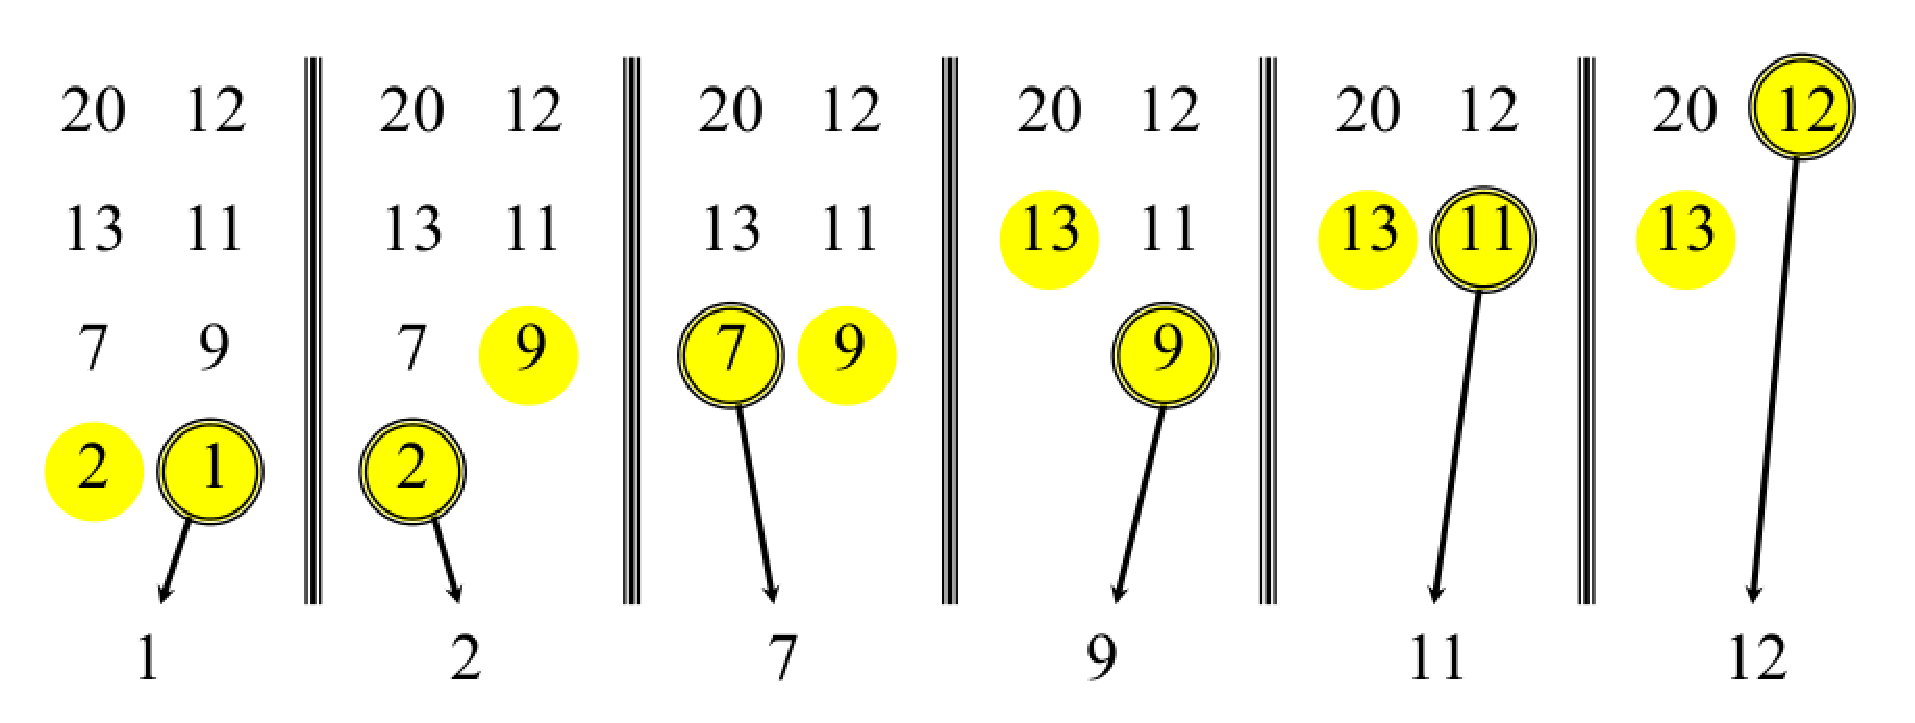
\includegraphics[width=4in]{lecture3/merge.eps}
  \caption{Процедура объединения}
  \label{fig:merge}
\end{figure}

Псевдокод сортировки:
\begin{codebox}
\Procname{$\proc{Merge\_Sort}(A, p, r)$}
  \li \If $p < r$
  \li \Then $q \gets \lfloor (p+r)/2 \rfloor$
  \li       $Merge\_Sort(A, p, q)$
  \li       $Merge\_Sort(A, q+1, r)$
  \li       $Merge(A, p, q, r)$
      \End
\end{codebox}

Анализируя, получаем рекуррентность $T(n) = 2T(n/2) + \Theta(n)$. Её решением,
согласно второму случаю основной теоремы, будет $\Theta(n log(n))$

\section{Основная теорема}
При использовании основного метода функция $f(n)$ сравнивается с $n^{\log_b a}$
и рассматриваются три случая. Интуитивно понятно, что асимптотическое поведение
решения рекуррентного соотношения определяется большей из двух функций.

\begin{enumerate}
\item Если $f(n) = O(n^{\log_{b}{a - \epsilon}})$ , для некоторой константы
  $\epsilon > 0$, т.е. $f(n)$ растет полиноминально медленней, чем
  $n^{\log_b a}$ в $n^\epsilon$ раз.\\
  Тогда $T(n) = \Theta(n^{\log_b a})$

\item Если $f(n) = \Theta(n^{\log_b a}\lg^k n)$, т.е. $f(n)$ и $n^{log_b a}$
  растут с одинаковой скоростью с точностью до множителя $\lg^k n$, для
  константы $k \geqslant 0$.\\ Тогда $T(n) = \Theta(n^{\log_b a} \lg^{k+1} n)$

\item Если $f(n) = \Omega(n^{\log_b{a + \epsilon}})$ , для некоторой константы
  $\epsilon > 0$, т.е. $f(n)$ растет полиноминально быстрей, чем $n^{\log_b a}$
  в $n^\epsilon$ раз \\ \emph{и} $f(n)$ удовлетворяет неравенству $a f(n/b)
  \leqslant c f(n)$ для некоторого $c < 1$ \\ Тогда $T(n) = \Theta(f(n))$
\end{enumerate}

В сортировке слиянием $a = 2, b = 2, f(n) = \Theta(n)$, то есть нам нужно
сравнить $\Theta(n)$ и $n^{\log_2 2} = n^1 = n$. Они апроксиматически равны
(случай 2 теоремы, $k = 0$), таким образом, ответом будет $T(n) = \Theta(n \lg
n)$

\section{Бинарный поиск}
Другим примером метода ``разделяй и властвуй'' является бинарный поиск.

Оценка времени выполнения: $T(n) = T(n/2) + \Theta(1)$ (одно подзадача в два
раза меньше основной задачи и константное время для объединения), снова второй
случай основной теоремы и решение $T(n) = \Theta(\lg n)$

\section{Возведение в степень}
Задача: найти целую степень числа, то есть найти $a^n, \text{ где } n \in
\mathbb{N}$. Наивный алгоритм решает задачу за  $\Theta(n)$. Алгоритм ``разделяй
и властвуй'' даёт лучшее решение:

\begin{equation*}
  a(n) = \begin{cases}
    a^{n/2} a^{n/2}, \text{ если n -- чётное} \\
    a^{(n-1)/2} a^{(n-1)/2} a,  \text{ если n -- нечётное}
  \end{cases}
\end{equation*}

Время работы: $T(n) = T(n/2) + \Theta(1) \Rightarrow T(n) = \Theta(\lg n)$

\section{Числа Фибоначчи}

Рекурсивное определение:
\begin{equation*}
  F_n = \begin{cases}
    0, \text{ если } n = 0 \\
    1, \text{ если } n = 1 \\
    F_{n-1} + F_{n-2}, \text{ если } n > 1
  \end{cases}
\end{equation*}

Наивный рекурсивный алгоритм: $\Omega(\phi^n)$, где $\phi$ -- золотое сечение.
Экспоненциальное время работы -- очень плохо.

Итеративный алгоритм: последовательно считать $F_0, F_1, F_2, \ldots$ для
получения нового числа складывать два предыдущих -- на каждое число одно
сложение, значит время выполнение $T(n) = \Theta(n)$

Наивное возведение в степень: мы можем использовать известную формулу $F_n =
\phi^n / \sqrt{5}$, округлённое в сторону ближайшего целого. Используя оценку из
предыдущего раздела, получим время выполнения $\Theta(\lg n)$. Однако этот метод
не слишком надёжный, т.к. из-за ошибок округления вещественных чисел можем
получить неверный результат.

Теорема:
\begin{equation*}
\begin{bmatrix}
  F_{n+1} & F_n \\
  F_n     & F_{n-1}
\end{bmatrix} =
\begin{bmatrix}
  1 & 1 \\
  1 & 0
\end{bmatrix}^n
\end{equation*}

Алгоритм: рекурсивное возведение в квадрат (то же, что применялось для
возведения в степень). Его оценка, как известно $\Theta(\lg n)$.
Возведение матрицы 2 на 2 в квадрат асимптотически ничем не отличается от
возведения числа в квадрат, просто вместо одного умножения придётся делать
восемь и ещё четыре сложения, но все равно константное время $\Theta(1)$

Доказательство теоремы (индукция по $n$):
Базис ($n=1$)
\begin{equation*}
\begin{bmatrix}
  F_2 & F_1 \\
  F_1 & F_0
\end{bmatrix} =
\begin{bmatrix}
  1 & 1 \\
  1 & 0
\end{bmatrix}^1
\end{equation*}

Индукция (для $n > 1$):
\begin{equation*}
\begin{bmatrix}
  F_{n+1} & F_n \\
  F_n     & F_{n-1}
\end{bmatrix} =
\begin{bmatrix}
  F_n     & F_{n-1} \\
  F_{n-1} & F_{n-2}
\end{bmatrix}
\begin{bmatrix}
  1 & 1 \\
  1 & 0
\end{bmatrix} =
\begin{bmatrix}
  1 & 1 \\
  1 & 0
\end{bmatrix}^{n-1}
\begin{bmatrix}
  1 & 1 \\
  1 & 0
\end{bmatrix} =
\begin{bmatrix}
  1 & 1 \\
  1 & 0
\end{bmatrix}^n
\end{equation*}

\section{Умножение матриц}
Вход: $A = [a_{ij}], B = [b_{ij}]$

Выход: $C = [c_{ij}] = A \cdot B, i \in 1 \ldots n$

\begin{equation*}
\begin{pmatrix}
c_{11} & c_{12} & \ldots & c_{1n} \\
c_{21} & c_{22} & \ldots & c_{2n} \\
\vdots & \vdots & \ddots & \vdots \\
c_{n1} & c_{n2} & \ldots & c_{nn}
\end{pmatrix}
=
\begin{pmatrix}
a_{11} & a_{12} & \ldots & a_{1n} \\
a_{21} & a_{22} & \ldots & a_{2n} \\
\vdots & \vdots & \ddots & \vdots \\
a_{n1} & a_{n2} & \ldots & a_{nn}
\end{pmatrix}
\cdot
\begin{pmatrix}
b_{11} & b_{12} & \ldots & b_{1n} \\
b_{21} & b_{22} & \ldots & b_{2n} \\
\vdots & \vdots & \ddots & \vdots \\
b_{n1} & b_{n2} & \ldots & b_{nn}
\end{pmatrix}
\end{equation*}

Формула для нахождения элементов матрицы произведения:
\begin{equation*}
  c_{ij} = \sum_{k=1}^n a_{ik} b_{kj}
\end{equation*}

Наивный алгоритм на псевдокоде:
\begin{codebox}
\li \For $i \gets 1 $ \To $n$
\li     \Do \For $j \gets 1 $ \To $n$
\li         \Do $c_{ij} \gets 0$
\li             \For $k \gets 1 $ \To $n$
\li             \Do $c_{ij} \gets c_{ij} + a_{ik} b_{kj}$
                \End
            \End
        \End
\end{codebox}

Три вложенных цикла, т.е. сложность алгоритма будет $\Theta(n^3)$. Рассмотрим
алгоритм в стиле ``разделяй и властвуй''. Идея: представим, что матрица 
$n \times n$ -- это $2 \times 2$-матрица $(n/2) \times (n/2)$ подматриц:

\begin{equation*}
\begin{split}
\begin{bmatrix}
  r & s \\
  t & u
\end{bmatrix}
&=
\begin{bmatrix}
  a & b \\
  c & d
\end{bmatrix}
\cdot
\begin{bmatrix}
  e & f \\
  g & h
\end{bmatrix} \\
C &= A \cdot B
\end{split}
\end{equation*}

\begin{equation*}
\text{ 8 \emph{рекурсивных} умножений + 4 сложения матриц } 2 \times 2
\begin{cases}
  r = ae + bg \\
  s = af + bh \\
  t = ce + dg \\
  u = cf + dh
\end{cases}
\end{equation*}

Получим рекуррентность: $T(n) = 8T(n/2) + \Theta(n)$

Нужно сравнить $n^{\log_2 8}$ и $\Theta(n)$. Первое полинамильно больше,
получаем первый случай основной теоремы и, стало быть, решение: $T(n) =
\Theta(n^3)$

Решение оказалось точно таким же, как и оригинальное.

\section{Алгоритм Евклида}
Наибольший общий делитель (НОД) двух чисел $m$ и $n$ обычно обозначается как
\begin{equation*}
  gcd(m, n)
\end{equation*}
Если $gcd(m, n) = 1$, то числа $m$ и $n$ называются \emph{взаимно простыми}.
Кроме того, $gcd(n, 0) = n$ для любого $n > 0$.

Первый из известных алгоритмов нахождения НОД описан Евклидом в книге 
``Начала'' (около 300 г. до н.э.). Он записывается рекурсивной формулой:
\begin{codebox}
\Procname{$\proc{Euclid}(m, n)$}
  \li \If $n = 0$
  \li \Then \Return $m$
  \li \Else \Return $Euclid(n, m \bmod n)$
      \End
\end{codebox}

Идея заключается в том, что НОД двух чисел не изменится, если из большего числа
вычесть меньшее. Т.е. если $21$ -- НОД $252$ и $105$, то $205-105 = 147$ и
$21$ по-прежнему является НОД $147$ и $105$. Остаток от последовательного 
вычитания второго аргумента из первого и выражается формулой $m \bmod n$.

Работа этого рекурсивного алгоритма не может продолжаться до бесконечности,
т.к. второй аргумент функции всегда строго убывает, и он всегда неотрицательный.
Таким образом, результатом всегда будет правильный ответ.

Существует другой метод поиска НОД, где операции умножения и деления заменены
операциями бинарного сдвига. Этот метод обычно работает быстрее, т.к. сдвиг
намного дешевле других операций. Алгоритм бинарного НОД был известен ещё в
Китае в первом веке н.э., но опубликован был лишь в 1967 году израильским 
программистом Джозефом Стайном. Метод использует следующие свойства НОД:

\begin{enumerate}
\item $gcd(0, n) = n$; $gcd(m, 0) = m$; $gcd(m, m) = m$ -- по определению gcd
\item Если $m$, $n$ чётные, то $gcd(m, n) = 2*gcd(m/2, n/2)$, т.к. 2 -- общий 
  делитель
\item Если $m$ чётное, $n$ нечётное, то $gcd(m, n) = gcd(m/2, n)$, т.к. 2 -- не
  общий делитель
\item Если $n$ чётное, $m$ нечётное, то $gcd(m, n) = gcd(m, n/2)$
\item Если $m$, $n$ нечётные и $n > m$, то $gcd(m, n) = gcd((n - m)/2, m)$ -- 
  комбинация из одного шага простого алгоритма Евклида (вычитания) и шагов 3-4
  бинарного алгоритма
\item Если $m$, $n$ нечётные и $n < m$, то $gcd(m, n) = gcd((m - n)/2, n)$
\end{enumerate}

Шаги повторяются, пока не будет $m = n$, а затем ещё раз, пока $n = 0$.
Определение алгоритма рекурсивно, но это хвостовая рекурсия, а значит её
можно заменить итерацией.

Время работы алгоритма $O(\log^2 m n)$, т.е. пропорционально квадрату
количества бит $m$ и $n$ вместе.

Существуют расширенные версии обоих вариантов алгоритмов, которые параллельно с
НОД вычисляют полезные константы $a$ и $b$, где
\begin{equation*}
  a m + b n = gcd(a, b)
\end{equation*}

Наибольший общий делитель двух чисел имеет ряд важных применений в криптографии
с открытым ключём, в решении Диофантовых уравнений и в ряде других задач
теории чисел.

\section*{Заключение}
\begin{itemize}
\item ``Разделяй и властвуй'' -- одна из нескольких мощных техник для разработки
  алгоритмов
\item Оценка времени выполнения этих алгоритмов сводится к рекуррентностям,
  которые легко решаются основной теоремой
\item Стратегия ``Разделяй и властвуй'' часто позволяет получить весьма
  эффективные алгоритмы
\end{itemize}
\end{document}
